\documentclass[11pt]{article}
\usepackage[a4paper, margin=2.5cm]{geometry}

\usepackage[slovene]{babel}
\usepackage[utf8]{inputenc}
\usepackage[T1]{fontenc}
\usepackage{lmodern}

\usepackage{xcolor} 

\usepackage{url}
\usepackage{graphicx}
\usepackage{amsmath}
\usepackage{amsthm}
\usepackage{amssymb}

\usepackage{booktabs}
\usepackage{siunitx}

\newcommand{\m}{\mathcal{F}}

\theoremstyle{definition}
\newtheorem{definicija}{Definicija}

\theoremstyle{plain}
\newtheorem{izrek}{Izrek}

\title{Brownovo gibanje}
\author{Matej Rojec}
\date{}

\begin{document}

\maketitle

Brownovo gibanje (več v~\cite{karatzas1991brownian}) je intuitivno slučajen proces, % Sklic na knjigo
ki predstavlja naključno gibanje delcev v mediju.

\begin{figure}[!ht]
    \centering
    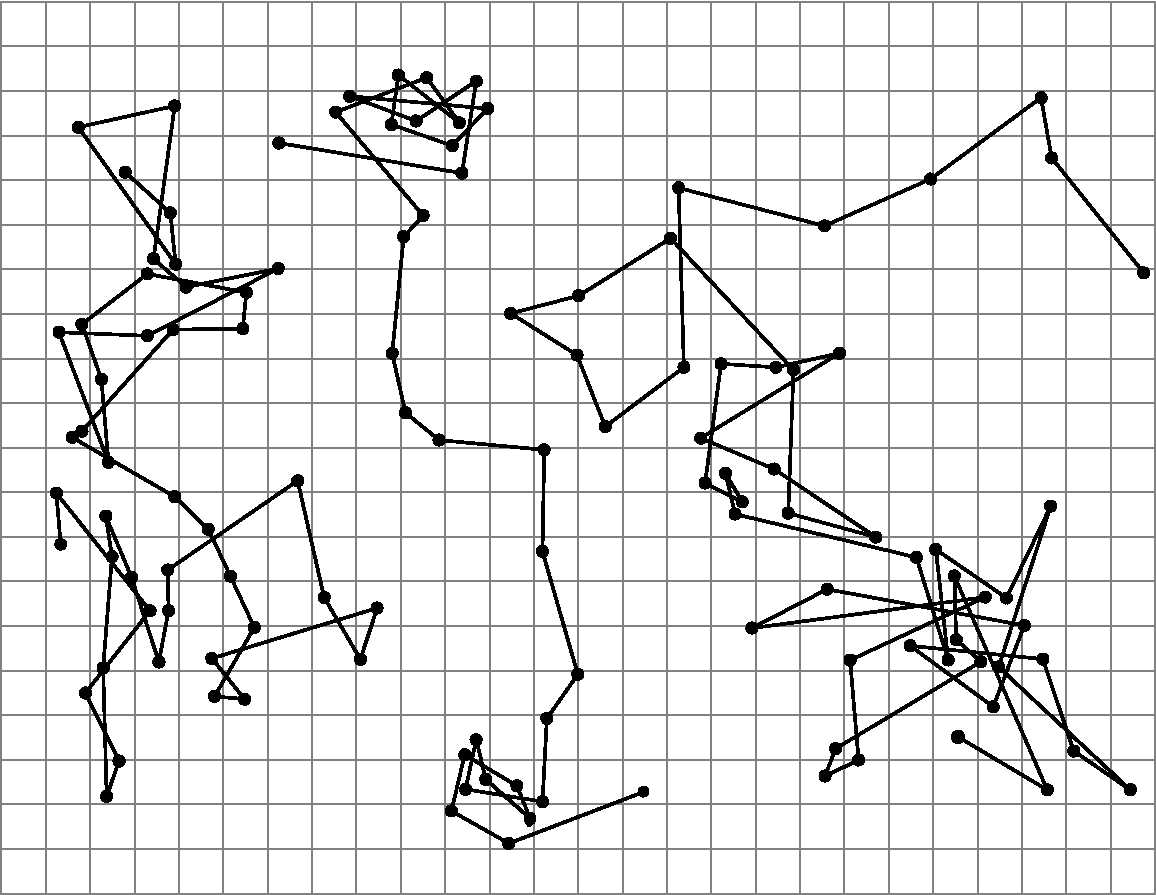
\includegraphics[scale=0.33]{PerrinPlot2.pdf}
    \caption{Reprodukcija slike iz Jean Baptiste Perrin, \emph{Mouvement brownien et réalité moléculaire}, Ann. de Chimie et de Physique (VIII) 18, 5-114, 1909}
  \label{fig:Perrin}
\end{figure}
    % Slika: PerrinPlot2.pdf, velikost scale=0.3
    % Napis pod sliko: 
    % Reprodukcija slike iz Jean Baptiste Perrin, \emph{Mouvement brownien et réalité moléculaire}, Ann. de Chimie et de Physique (VIII) 18, 5-114, 1909

    % Začetek definicije
    
    \begin{definicija}
        \emph{Standardno Brownovo gibanje} \(\{B_t\}_{t \geq 0}\) je slučajen proces z naslednjimi lastnostmi: 
            \begin{enumerate}
                \item \(B_0 = 0\).
                \item Prirastki \(B_{t_n} - B_{t_{n-1}}, B_{t_{n-1}} - B_{t_{n-2}}, \ldots, B_{t_2} - B_{t_1}, B_{t_1} - B_{t_0}\) so neodvisne slučajne spremenljivke, za vsak \(t_0 \leq t_1 \leq \cdots \leq t_{n-1} \leq t_n\).
                \item Za vsak \(t \geq 0\) in \(h > 0\) velja \(B_{t+h} - B_t \sim \mathcal{N}(0, h)\).
                \item Funkcija \(t \mapsto B_t\) je zvezna skoraj gotovo.
            \end{enumerate}
    \end{definicija}
    % Konec definicije
    
    Preden zapišemo izrek, definirajmo še pojem časa ustavljanja.
    
    % Začetek definicije
    
    \begin{definicija}
        Slučajna spremenljivka \(\tau\) na verjetnostnem prostoru \((\Omega, \m, P)\) z vrednostmi v \(\mathbb{R}^+\)
        je \emph{čas ustavljanja glede na filtracijo} \((\m_t)_{t\in T}\), če velja: \(\forall t\in T : \{\tau \leq t\} \in \m_t\).
    \end{definicija}
    % Konec definicije
    
    Zdaj lahko zapišemo izrek~\ref{thm:stopped_brownian}. % Sklic na izrek z oznako thm:stopped_brownian
    
    % Začetek izreka
    
    \begin{izrek}
        \label{thm:stopped_brownian}
            Naj bo \(\{B_t\}_{t \geq 0}\) (standardno) Brownovo gibanje, \(\tau\) čas ustavljanja glede na
            \((\m_t)_{t \geq 0}\) in naj velja \(P [\tau < \infty] = 1\).
            Potem je tudi proces:
            \[
            \hat{B} := \{B_{\tau+t} - B_\tau \mid t \geq 0\}
            \]
            (standardno) Brownovo gibanje in neodvisen od \(\m_\tau\).
    \end{izrek}
    % Konec izreka


\bibliographystyle{plain}
\bibliography{knjiga}

\end{document}